\documentclass[a4paper,11pt]{article}
\usepackage{zh_CN-Adobefonts_external}
\usepackage{fancyhdr}  % 页眉页脚
\usepackage{minted}    % 代码高亮
\usepackage[colorlinks]{hyperref}  % 目录可跳转
\usepackage{ulem} % 支持删除
\usepackage{amsmath}
\usepackage{longtable,booktabs}
\usepackage{graphics} % 插入图片
\setlength{\headheight}{15pt}

% 定义页眉页脚
\pagestyle{fancy}
\fancyhf{}
\fancyhead[C]{Algorithm Library by lonlyn}
\lfoot{}
\cfoot{\thepage}
\rfoot{}

\author{lonlyn}   
\title{Algorithm Library}

\begin{document} 
\maketitle % 封面
\newpage % 换页
\tableofcontents % 目录
\newpage
\setcounter{page}{1}
% 基础类start
\section{基础类} 
\subsection{常用函数与类模板}
\subsubsection{二分查找}
\paragraph{lower\_bound()}
第一个\textbf{大于等于}值的元素的位置
\paragraph{upper\_bound()}
第一个\textbf{大于}值的元素的位置
\subsubsection{二进制}
\paragraph{\_\_builtin\_ffs(x)}
返回 x 的最后一位 1 是从后往前第几位
\paragraph{\_\_builtin\_clz(x)}
返回 x 的二进制下前导 0 个数
\paragraph{\_\_builtin\_ctz(x)}
返回 x 的二进制下末尾 0 个数
\paragraph{\_\_builtin\_popcount(x)}
返回 x 的二进制下 1 的个数
\paragraph{\_\_builtin\_parity(x)}
返回 x 的二进制下 1 的个数的奇偶性
\subsection{快速输入,输出} % 二级标题
注:I\_int 后面的元素根据实际更改即可
\inputminted[linenos]{c++}{basic/inout.cpp}
% string模板
\subsection{string}
getline(cin,str) 读取一行并存储在str。(需要引用string库)

begin(),end() 起始/末尾的迭代器

empty(),size(),length() 是否为空及长度

insert(pos,count,ch) 在pos插入count个ch

insert(pos,str) 在pos插入str

erase(first,last) 删除 [first,last) 的字符串

push\_back(),pop\_back() 后附/移除末尾字符

append(str) 末尾添加字符串

% 高精度
\subsection{高精度}
\inputminted[linenos]{c++}{basic/high.cpp}
% 离散化
\subsection{离散化}
\inputminted[linenos]{c++}{basic/discretization.cpp}

% STL start
\subsection{C++ STL}
\subsubsection{序列式容器:vector,deque,list}
% vector
\textbf{(1)vector:}

构造:

\textbf{vector\textless{}int\textgreater{} a; }

\textbf{vector\textless{}int\textgreater{} a(size{[},value{]});}
创建有size个元素的vector并把value作为初值(默认0)。

访问与修改:

注:所有增减元素在中间的线性复杂度是根据操作位置与\textbf{最后元素}的距离而言的。

\textbf{a.assign(size,const T\& value)} 将size份value覆盖到a里。
\(O(n)\)

\textbf{a.begin() a.end()}
返回起始地址和\textbf{末元素后一位}的元素的地址。

\textbf{a.clear()} 将a中元素全部擦除。 \(O(n)\)

\textbf{a.insert(iterator pos,const T\&value)}
在pos前插入value。\(O(n)\)

\textbf{a.erase(iterator pos) } 删除pos处元素。\(O(n)\)

\textbf{a.erase(iterator first,iterator last)} 删除{[}first;last)
中的元素。\(O(n)\)
% deque
\noindent\textbf{(2)deque:}

构造:

\textbf{deque\textless{}int\textgreater{} a; }

\textbf{deque\textless{}int\textgreater{} a(size{[},value{]});}
创建有size个元素的deque并把value作为初值(默认0)。

访问与修改:

注:所有增减元素在中间的线性复杂度是根据操作位置与\textbf{两端最近的}距离而言的。

\textbf{a.front(); a.back();} 返回头/尾元素的值。

\textbf{clear insert erase begin end} 同上

\textbf{a.push\emph{front(const T\& value); a.push}back(const T\&
value);} 头部与末尾插入元素。

\textbf{a.pop\emph{front(); a.pop}back(const T\& value);}
头部与末尾弹出元素。
% list
\noindent\textbf{(3)list:}

构造:

\textbf{list\textless{}int\textgreater{} a; }

\textbf{list\textless{}int\textgreater{} a(size{[},value{]});}
创建有size个元素的list并把value作为初值(默认0)。

访问与修改:

\textbf{a.front(); a.back();} 返回头/尾元素的值。

\textbf{a.begin() a.end()}
返回起始地址和\textbf{末元素后一位}的元素的地址。

\textbf{a.clear()} 将a中元素全部擦除。复杂度 \(O(n)\)

\textbf{a.insert(iterator pos,const T\&value)}
在pos前插入value。\(O(1)\)

\textbf{a.erase(iterator pos) } 删除pos处元素。\(O(1)\)

\textbf{a.erase(iterator first,iterator last)} 删除{[}first;last)
中的元素。

\textbf{a.push\emph{front(const T\& value); a.push}back(const T\&
value);} 头部与末尾插入元素。

\textbf{a.pop\emph{front(); a.pop}back(const T\& value);}
头部与末尾弹出元素。

\textbf{a.sort({[}comp{]});} 排序,comp为\textbf{bool comp(const Type
\&\_a,const Type \&b)\{\}}\(O(n\log n)\)

\textbf{a.reverse();} 翻转顺序。 \(O(n)\)

\textbf{a.unique();} 去除所有\textbf{相继}的重复元素。 \(O(n)\)

\textbf{a.merge(list b{[},comp{]});}
合并\textbf{有序列表}a,b(归并排序)。\(O(n)\)

\subsubsection{关联式容器:(multi)set,(multi)map}
% set
\textbf{(1)set:}

构造:

\textbf{set\textless{}Type\textgreater{} a;}

\textbf{set\textless{}Type,TypeComp\textgreater{} a; }

注:这里的TypeComp需为struct而不是operator。如:
\inputminted[linenos]{c++}{basic/typecomp.cpp}


访问与修改:

\textbf{a.clear()} 清空元素。\(O(n)\)

\textbf{a.insert(value)} 插入元素。\(O(\log n)\)

\textbf{a.erase(iterator pos)} 清除位于pos的元素。\(O(1)\)

\textbf{a.erase(const key\_type\& key);}
清除关键等于key的元素。\(O(\log n)\)

\textbf{a.count(value)} 返回是否存在该元素(0/1)。 \(O(\log n)\)

\textbf{a.find(value)}
返回值为value的元素的\textbf{迭代器},没有则为a.end()。\(O(\log n)\)

\textbf{a.lower\_bound(value)}
返回指向首个\textbf{不小于}value的迭代器。\(O(\log n)\)

\textbf{a.upper\_bound(value)}
返回指向首个\textbf{大于}value的迭代器。\(O(\log n)\)
% multiset
\noindent\textbf{(2)multiset:}

构造:

与set相似。略。

访问与修改:(与set功能相同的已经省略)

\textbf{a.erase(const key\_type\& key);}
清除关键字等于key的\textbf{所有}元素。\(O(\log n+a.count(key))\)

\textbf{a.count(value)} 返回键值为key的元素有多少个。 \(O(\log n)\)

% map
\noindent\textbf{(3)map:}

构造:

\textbf{map\textless{}Type1 a,Type2 b\textgreater{} mp;}

\textbf{map\textless{}Type1 a,Type2 b,Type1Comp\textgreater{} mp;}

这里的Type1Comp是针对Type1的,且需为struct而不是operator。

访问与修改:

\textbf{mp.clear()} 清除。\(O(n)\)

\textbf{mp.insert(pair\textless{}Type1,Type2\textgreater{}(a,b));
}添加元素,不过可以直接mp{[}Type1{]}=Type2。\(O(\log n)\)

如果重复插入相同键值(Type1)则\textbf{后序插入的被忽略}。

\textbf{mp.insert\emph{or}assign(pair\textless{}Type1,Type2\textgreater{}(a,b));}
添加元素,\(O(\log n)\)

如果重复插入相同键值(Type1)则\textbf{后序插入值覆盖原来的值}。

\textbf{mp.erase(iterator pos)} 清除位于pos的元素。\(O(1)\)

\textbf{mp.erase(iterator first,iterator last);
}清除{[}first;last)的元素。

\textbf{mp.erase(const key\_type\& key);}
清除关键等于key的元素。\(O(\log n)\)

\textbf{mp.count(const Key\& key);}
返回键值为key的元素个数(0/1)。\(O(\log n)\)

\textbf{mp.find(const Key\& key);}
返回键值为key的元素的iterator。否则mp.end()。\(O(\log n)\)

\textbf{mp.lower\_bound(const Key\& key);}
返回首个\textbf{不小于}k的键值所在元素的iterator。

\textbf{mp.upper\_bound(const Key\& key);}
同上,不过是\textbf{大于}。两者 \(O(\log n)\)
% multimap
\noindent\textbf{(4)multimap:}

因为 multimap 允许多个元素拥有同一键的特点,multimap
并\textbf{没有提供给出键访问其对应值的方法}。

构造:

同map构造。

访问及修改(不同的):

\textbf{mp.erase(const key\_type\& key);}
清除关键等于key的\textbf{所有}元素。\(O(\log n)\)

\textbf{mp.count(const Key\& key);}
返回键值为key的元素个数。\(O(\log n)\)

\subsubsection{无序关联式容器:unrodered\_(multi)set,map} 
所有元素哈希处理。但遇到cf赛事时注意防卡hash。

% unordered set
\noindent\textbf{(1)unordered\_set:}

构造:

\textbf{unordered\_set\textless{}Type\textgreater{} st;}

\textbf{unordered\_set\textless{}Type,Hash,Keyequal\textgreater{} st;}

Type表示类型,Hash表示哈希方法,Keyequal表示判定键值相同方法。后两者用struct判断。

如果Type不是自定义类型的话就不用写Keyequal,或者写上更难hack。

下面给出一个hash与equal栗子(摘自OI-Wiki)
\inputminted[linenos]{c++}{basic/hashequal.cpp}

\noindent\textbf{(2)unordered\_multiset:}

同上,不多赘述。

\noindent\textbf{(3)unordered\_map:}

构造:

\textbf{unordered\_map\textless{}Type1,Type2\textgreater{} mp;}

\textbf{unordered\_map\textless{}Type1,Type2,Type1Hash,Type1Equal\textgreater{};}

Type1Hash与Type1Equal规则和上文一样。不再赘述。

\noindent\textbf{(4)unordered\_multiset:}

同上,不多赘述。

% 基础类end

\newpage
% 数论begin
\section{数论}
\subsection{数论相关定理和规律}
\begin{itemize}
\item
  费马小定理:当 \(a,p\in Z\) 且 \(p\) 为质数,且
  \(a\not\equiv 0\ (mod\ p)\) ,有 \(a^{p-1}\equiv 1\ (mod\ p)\) 。所以
  \(a^b\equiv a^{b\ mod\ (p-1)}\ (mod\ p)\) 。
\item
  欧拉定理:当 \(a,m\in Z\) ,且 \(gcd(a,m)=1\) 时,有
  \(a^{\varphi(m)}\equiv 1\ (mod\ m)\) 。所以
  \(a^b\equiv a^{b\ mod\ \varphi(m)}\ (mod\ m)\) 。 
\item
  扩展欧拉定理:不需要互质啦:

  \begin{equation}
  a^c \equiv
  \begin{aligned}
  &a^{c\ mod\ \varphi(m)}&,{gcd(a,m)=1}\\
  &a^c&,gcd(a,m)\not=1,c<\varphi(m)\\
  &a^{(c\ mod\ \varphi(m))+\varphi(m)}&,{gcd(a,m)\not=1,c\ge\varphi(m)}\\
  \end{aligned}
  \end{equation}
\item
  二项式定理:\((x+y)^n=\sum\limits_{k=0}^{n}{C_{n}^{k}x^{n-k}y^k}\)
\item
  第二类斯特林数 \(S(n, k)\):将 \(n\) 个互不相同的元素分成 \(k\) 个互不区分非空子集的方案数。
  如果区分先后子集,注意乘上阶乘。
  
  \(S(n,0) = [n=0]\)
  
  \(S(n,k)=S(n-1,k-1)+k\times S(n-1, k)\)

  \(S(n,k)=\sum\limits_{i=0}^{m}{\frac{(-1)^{m-i}i^n}{i!(m-i)!}}\)
\item
  错排公式:

  \begin{itemize}
  \item
    递推公式:\(D(n) = (n-1) [D(n-2) + D(n-1)]\),特殊的,\(d[1]=0,d[2]=1\)。关于
    \(d[0]\) 的取值:如果参与乘法运算考虑是否更改为 \(1\),正常情况为
    \(0\)。
  \item
    整体公式:\(D(n) = n! [\frac{1}{0!} - \frac{1}{1!} + \frac{1}{2!} - \frac{1}{3!} + \frac{1}{4!} + ... + \frac{(-1)^n}{n!}]\)
  \item
    简化公式:\(D(n) = \lfloor \frac{n!}{e}+0.5\rfloor\)
  \end{itemize}
\item
  卢卡斯定理:\(\dbinom{n}{m}\bmod p=\dbinom{\lfloor n/p\rfloor}{\lfloor m/p\rfloor}\cdot\dbinom{n\bmod\ p}{m\bmod\ p}\bmod p\)
\item
  \(\sum\limits_{d|n}{\mu(d)}=[n=1],\mu\ *\ I=\epsilon\),\(\sum\limits_{d|n}{\varphi(d)}=n,\varphi\ *\ I=id\)
\item
  同余问题难以解决时,考虑移项。遇到倍数问题,尝试同除 gcd 得到互质,从而消去(乘互质的数对倍数无贡献)。
\item
  \((a\ and\ b)*2=(a\ xor\ b)+(a+b)\)
\item
  二阶线性递推数列:\(x_n=a_1x_{n-1}+a_2x_{n-2}\) 的特征方程是 \(x^2-a_1x-a_2=0\) 。求得两个解后,通项为 \(x_n=c_1{x_1}^n+c_2{x_2}^n\) ,\(c_1,c_2\) 通过带入求解。例如斐波那契数列 \(x_n=x_{n-1}+x_{n-2}\) ,特征方程 \(x^2-x-1=0\) ,求出两个解,同时带入特殊值即可求出通项: \(\frac{1}{\sqrt{5}}[(\frac{1+\sqrt{5}}{2})^n-(\frac{1-\sqrt{5}}{2})^n]\)
\item
  n个数快速因式分解:如果在值域较小的情况下,预处理d[i]数组代表i的最小质因子,省去挪指针的时间。例求解35的因子,d[35]=5,d[35/5]=d[7]=[7],便得到了35包含的质因子3,7。
\item 
  低阶等幂求和公式:
  \begin{enumerate}
    \item $\sum\limits_{i=1}^{n}{i^1}=\frac{n(n+1)}{2}=\frac{1}{2}n^2+\frac{1}{2}n$
    \item $\sum\limits_{i=1}^{n}{i^2}=\frac{n(n+1)(2n+1)}{6}=\frac{1}{3}n^3+\frac{1}{2}n^2+\frac{1}{6}n$
    \item $\sum\limits_{i=1}^{n}{i^3}=\left[\frac{n(n+1)}{2}\right]^2=\frac{1}{4}n^4+\frac{1}{2}n^3+\frac{1}{4}n^2$
    \item $\sum\limits_{i=1}^{n}{i^4}=\frac{n(n+1)(2n+1)(3n^2+3n-1)}{30}=\frac{1}{5}n^5+\frac{1}{2}n^4+\frac{1}{3}n^3-\frac{1}{30}n$
    \item $\sum\limits_{i=1}^{n}{i^5}=\frac{n^2(n+1)^2(2n+1)(2n^2+2n-1)}{12}=\frac{1}{6}n^6+\frac{1}{2}n^5+\frac{5}{12}n^4-\frac{1}{12}n^2$
  \end{enumerate}

\end{itemize}
% 线性筛
\subsection{线性筛}
\inputminted[linenos]{c++}{math/linear.cpp}
% 逆元
\subsection{逆元}
\subsubsection{单个逆元}
\[a^{p-2}\equiv \frac{1}{a}(mod\ p)\]
\subsubsection{线性阶乘逆元}
考虑到
\(\frac{1}{(n+1)!}\times (n+1)=\frac{1}{n!}\),求出最大的往下递推即可。
\subsubsection{线性逆元}
\inputminted[linenos]{c++}{math/niyuan1.cpp}
\subsubsection{任意n个数的逆元}
\inputminted[linenos]{c++}{math/niyuan2.cpp}
% exgcd
\subsection{Exgcd与线性同余方程}
\subsubsection{Exgcd}
返回一组满足\(ax+by=c\)的(x,y)
\inputminted[linenos]{c++}{math/exgcd.cpp}
\subsubsection{线性同余方程}
返回 \(x\)
满足\(ax\equiv c(mod\ b)\),转化为\(ax+by=c\)解决。有解需要满足\(gcd(a,b)|c\)
\inputminted[linenos]{c++}{math/tongyufangcheng.cpp}
% crt
\subsection{线性同余方程组及中国剩余定理}
\subsubsection{CRT}
求得\(x \equiv a_i(mod\ m_i)\)需要\textbf{保证模数\(m_1,m_2,\cdots ,m_n\)两两互质}。
\inputminted[linenos]{c++}{math/crt.cpp}
\subsubsection{EXCRT}
不保证两两互质也是可以的。
\inputminted[linenos]{c++}{math/excrt.cpp}
\subsubsection{StepMul}
\inputminted[linenos]{c++}{math/quickmul.cpp}
% bsgs
\subsection{BSGS}
求得 \(x\)
,使得\(a^x=b(mod\ p)\)。(\textbf{要求a,p互质,不一定p为质数})
\inputminted[linenos]{c++}{math/bsgs.cpp}

% 二次剩余
\subsection{二次剩余}
求解 \(x\) 使得 \(x^2 \equiv a \pmod p\),即模意义下开方。\(p\)
是奇素数。二次剩余有 \(\frac{p-1}{2}\) 个,非二次剩余有
\(\frac{p-1}{2}\) 个。

勒让德符号:\(\left(\frac{n}{p}\right)\) ,值为 \(1\) 时 \(n\) 是 \(p\)
的二次剩余且 \(n\not\mid p\),\(0\) 时 \(p\mid n\),\(-1\) 时 \(n\) 不是
\(p\) 的二次剩余且 \(n\not\mid p\)。

欧拉判别准则:\(\left(\frac{n}{p}\right)\equiv n^{\frac{p-1}{2}}\pmod p\),通过判断
\(n^{\frac{p-1}{2}}\equiv \pm 1 \pmod p\) 即可得知。
\paragraph{cipolla}
求解 \(x^2\equiv a\pmod p\),随机找到 \(a\) 满足 \(a^2-n\)
为\textbf{非二次剩余}(期望为 \(2\) 次),定义
\(i^2\equiv a^2-n\pmod p\)。虽然 \(a^2-n\)
不是二次剩余,可以扩范围到复数。

考虑到
\((a+b)^p\equiv a^p+b^p\pmod p\),\(i^p\equiv i\cdot (i^2)^{\frac{p-1}{2}}\equiv -i\pmod p\),\(a^p\equiv a \pmod p\)。可以得到结论:

\[x\equiv (a+i)^{\frac{p+1}{2}}\equiv n^{\frac{1}{2}}\pmod p\]

得知一个解以后,另一个解便是其模意义上的相反数 \(p-x\)。同时别忘了0的存在。
\inputminted[linenos,breaklines]{c++}{math/cipolla.cpp}
% lucas
\subsection{卢卡斯定理及其扩展}
\subsubsection{Lucas}
\paragraph{\texorpdfstring{Lucas定理:要求\textbf{p是质数}(实际应用要求p不算大,在\({10}^5\)左右)。}{Lucas定理:要求p是质数(实际应用要求p不算大,在\{10\}\^{}5左右)。}}
\[\dbinom{n}{m}\bmod p=\dbinom{\lfloor n/p\rfloor}{\lfloor m/p\rfloor}\cdot\dbinom{n\bmod p}{m\bmod p}\bmod p\]
(以下代码\textbf{p均为全局变量})
\inputminted[linenos]{c++}{math/lucas.cpp}
\subsubsection{ExLucas}
\paragraph{\texorpdfstring{扩展Lucas:\textbf{p可以不为质数:}}{扩展Lucas:p可以不为质数:}}
将p分解质因数:\(p={p_1}^{k_1}{p_2}^{k_2}\cdots{p_n}^{k_n}\),对于每个
\(C_n^m\equiv a_i \pmod {{p_i}^{k_i}}\) 可以构成一组中国剩余定理。
对于 \(C_n^m\bmod p^t\),转化考虑 \(n!\bmod p^t\) 的值。我们把所有 \(n\)
及其倍数的因子提出来,发现提出来的因子为
\(p^{\lfloor \frac{n}{p}\rfloor}\cdot(\lfloor \frac{n}{p}\rfloor)! \)
,可以递推计算。前半部分以 \(p^t\) 为周期,后半部分单独乘上即可。
\inputminted[linenos,breaklines]{c++}{math/exlucas.cpp}

% 数论分块
\subsection{数论分块}
\subsubsection{性质}
对于\(i \in \Big[x,\lfloor\dfrac{n}{\lfloor\dfrac{n}{x}\rfloor}\rfloor\Big]\),值
\(\lfloor\dfrac{n}{i}\rfloor = \lfloor\dfrac{n}{x}\rfloor\) 是相同的。

设 \(j=\lfloor\frac{n}{\lfloor\frac{n}{i}\rfloor}\rfloor\) ,有
\(j=\lfloor\frac{n}{\lfloor\frac{n}{i}\rfloor}\rfloor\le \frac{n}{\lfloor\frac{n}{i}\rfloor}<j+1\)
,所以 \(\lfloor\frac{n}{i}\rfloor\le \frac{n}{j}\),且
\(\frac{n}{j+1}<\lfloor\frac{n}{i}\rfloor\) 。\(j\) 为最大取值。

如果遇到 \(\sum i\times f[i]\) 的问题,考虑 \(f[i]\)
能否用数列性质得出。
\subsubsection{代码}
以下代码求解的是 \(\sum\limits_{i=1}^{n}{\left\lfloor \frac{n}{i}\right\rfloor}\) 。
\inputminted[linenos,breaklines]{c++}{math/fenkuai.cpp}
% mobius
\subsection{莫比乌斯反演}
\(a|b:b\ mod \ a=0\)

\[F(n)=\sum\limits_{d|n}f(d) \Rightarrow f(n)=\sum\limits_{d|n}\mu(d)F(\frac{n}{d})\]

\[F(n)=\sum\limits_{n|d}f(d) \Rightarrow f(n)=\sum\limits_{n|d}\mu(\frac{d}{n})F(d)\]

注(1):一般遇到\(\sum\limits_{i=1}^{n}\sum\limits_{j=1}^{m}[gcd(i,j)=d]\)的问题,我们一般设\(f(d)=\sum\limits_{i=1}^{n}\sum\limits_{j=1}^{m}[gcd(i,j)=d]\),然后设\(F(k)=\sum\limits_{i=1}^{n}\sum\limits_{j=1}^{m}[gcd(i,j)=k,2k,3k,\cdots]\),则显然\(F(k)=\sum\limits_{k|d}f(d)\)。又因为\(F(k)=\lfloor \frac{n}{k}\rfloor \cdot \lfloor \frac{m}{k}\rfloor\)容易得出,所以答案\(f(d)=\sum\limits_{d|k}\mu(\frac{k}{d})\cdot \lfloor \frac{n}{k}\rfloor \cdot \lfloor \frac{m}{k}\rfloor\)可以方便求出。

注(2):为了方便我们一般把\(\sum\limits_{i=1}^{n}\sum\limits_{j=1}^{m}[gcd(i,j)=d]\)的问题转化为
\(\sum\limits_{i=1}^{\lfloor \frac{n}{d} \rfloor}\sum\limits_{j=1}^{\lfloor \frac{m}{d} \rfloor}[gcd(i,j)=1]\)的问题,求解\(f(1)=\sum\limits_{k=1}^{min(n,m)}\mu(k)\cdot \lfloor \frac{n}{kd}\rfloor \cdot \lfloor \frac{m}{kd}\rfloor\)

注(3):莫比乌斯函数的一个重要性质:\(\sum\limits_{d|n}{\mu(d)}=[n=1]\)
,在 gcd
不是非常裸(比如与其他项相乘)的时候,借助此性质巧妙转换:\(\sum\limits_{d|gcd(i,j)}{\mu(d)}=[gcd(i,j)=1]\),然后我们将枚举
gcd 的约数转化为枚举约数即可。

\subsubsection{mu函数及其前缀和}
\inputminted[linenos]{c++}{math/mu.cpp}
\subsubsection{数论分块计算答案前缀和}
计算完前缀和一般就能处理区间问题。
\(\sum\limits_{k=1}^{min(x,y)}\mu(k)\cdot \lfloor \frac{x}{kd}\rfloor \cdot \lfloor \frac{y}{kd}\rfloor\)为例。
\inputminted[linenos]{c++}{math/mobius.cpp}
% 亚线性筛
\subsection{亚线性筛}
% 积性函数
\subsubsection{积性函数}
\(\forall a\perp b,f(ab)=f(a)f(b)\),若对不互质的成立则为完全积性函数。

常见的积性函数:
\begin{longtable}[]{@{}ll@{}}
\toprule
公式 & 解释\tabularnewline
\midrule
\endhead
\(d(x)=\sum_{i|n}1\) & 约数个数\tabularnewline
\(\sigma(x)=\sum_{i|n}i\) & 约数和\tabularnewline
\(\varphi(x)=\sum_{i=1}^{x}{[gcd(x,i)=1]}\) & 欧拉函数\tabularnewline
\(\mu(x)\) & 莫比乌斯函数\tabularnewline
\(\epsilon(x)=[x=1]\) & 元函数(完全积性)\tabularnewline
\(I(x)=1\) & 恒等函数(完全积性)\tabularnewline
\(id(x)=x\) & 单位函数(完全积性)\tabularnewline
\bottomrule
\end{longtable}

积性函数的性质:若 \(f(x),g(x)\) 是积性函数,则以下函数也是积性函数。

\begin{enumerate}
  \item \(h(x)=f(x^p)\)
  \item \(h(x)=f^p(x)\)
  \item \(h(x)=f(x)g(x)\)
  \item \(h(x)=\sum\limits_{d|x}f(d)g(\frac{x}{d})\)
\end{enumerate}

% 杜教筛
\subsubsection{杜教筛}
使用条件:

\begin{enumerate}
  \item 复杂度 \(O(n^{\frac{2}{3}})\) 。
  \item \(f(x)\) 为积性函数。
  \item 能找到一个积性函数 \(g(x)\),设 \(h=f*g\),满足以下特点:
  \begin{enumerate}
    \item \(h(x)\) 的前缀和很好求。
  \end{enumerate}
\end{enumerate}

假设要计算
\(\sum\limits_{i=1}^{n}{f(i)}\)。我们设另外两个积性函数 \(h,g\) ,使得
\(h=f*g\) 。记 \(S(n)=\sum\limits_{i=1}^{n}f(i)\) ,求得
\(\sum\limits_{i=1}^{n}{h(i)}=\sum\limits_{d=1}^{n}g(d)\cdot S(\lfloor \frac{n}{d}\rfloor)\)
。进一步变形得到:

\[g(1)S(n)=\sum\limits_{i=1}^{n}(f*g)(i)-\sum\limits_{d=2}^{n}g(d)\cdot S(\lfloor \frac{n}{d} \rfloor)\]

如果 \(h(i)=(f*g)(i)\) 前缀和很好求得,那么对后面的式子进行整除分块,求
\(s(n)\) 复杂度就是 \(O(n^{\frac{2}{3}})\) 。下面给出栗子:

1.求 \(S(n)=\sum\limits_{i=1}^{n}{\mu(i)}\)

设 \(g\) 为 \(I\) ,则 \(h=f*g=\epsilon\) 。则
\(S(n)=1-\sum\limits_{d=2}^{n}{S(\lfloor \frac{n}{d}\rfloor)}\) 。

2.求 \(S(n)=\sum\limits_{i=1}^{n}{\varphi(i)}\) 。

设 \(g\) 为 \(I\) ,则 \(h=f*g=id\) 。则
\(S(n)=\sum\limits_{i=1}^{n}{i}-\sum\limits_{d=2}^{n}{S(\lfloor \frac{n}{d}\rfloor)}\)
。

3.求 \(S(n)=\sum\limits_{i=1}^{n}{i*\varphi(i)}\)

\(h(n)=\sum_{d|n}{d\cdot\varphi(d)}\cdot g(\frac{n}{d})\) 。考虑将 \(d\)
消去,不妨设 \(g=I\) ,则
\(h(n)=\sum_{d|n}{\varphi(d)}\cdot {n}=n\sum_{d|n}{\varphi(d)}=n^2\)
。所以:\(S(n)=\sum_{i=1}^{n}i^2-\sum_{d=2}^{n}d\cdot S(\lfloor\frac{n}{d}\rfloor)\)
。另外,\(1^2+2^2+3^2+\cdots+n^2=\frac{n(n+1)(2n+1)}{6}。\)

\textbf{具体实现:}

\begin{itemize}
\item
  先线性筛出前 \(n^{\frac{2}{3}}\) 项,剩余部分时间复杂度为
  \(O(\int_0^{n^{\frac{1}{3}}}{\sqrt{\frac{n}{x}}}\ dx)=O(n^{\frac{2}{3}})\)
\item
  剩下的东西Hash存储,或者直接unordered\_map(如果用map则多一个log)
\item
  注意取模以及\textbf{常数因子}的影响(过多的取模和long
  long的不必要使用)
\end{itemize}

以下代码是1,2问的。
\inputminted[linenos]{c++}{math/dujiaoshai.cpp}

% Min 25
\subsubsection{Min25筛}
使用条件:

\begin{enumerate}
  \item 复杂度 \(O(\frac{n^{\frac{3}{4}}}{\log n})\) 。
  \item \(f(x)\) 为积性函数。
  \item 设 \(p\) 为质数,则 \(f(p),f(p^c)\) 可以快速计算。
\end{enumerate}

\paragraph{过程}

\subparagraph{求解质数位置 \(f(x)\) 和} 
\leavevmode

设 \(p_k\) 为第 \(k\) 小的质数,约定 \(p_0=1\)。

设 \(s(n)\) 为 \(n\) 的最小质因子,约定 \(s(1)=1\)。

定义函数 \(f'(x)\),满足以下特点:
\begin{enumerate}
  \item \(f'(x)\) 是完全积性函数。
  \item 质数位置值与 \(f(x)\) 相同,即 \(\forall x\in {prime}, f(x) = f'(x)\)。
  \item \(f'(x)\) 可以快速求得前缀和。
\end{enumerate}

设 \(g(n,k)=\sum\limits_{i=2}^{n}{[isprime(i)\ or\ s(i)>p_k]f'(i)}\) ,
先预处理出所有的 \(g(n,0)=\sum\limits_{i=2}^{n}{f'(i)}\) 。

设 \(m\) 为 \(p_{m+1}>\sqrt{n}\) 的第一个位置,
那么 \(g(n,m)\) 就是所有质数的 \(f'(x)\) 和,
也即 \(f(x)\) 和。 

考虑写出 \(g(n,m)\) 的递推式:

\[
\begin{aligned}
  g(n,j)&=g(n,j-1)-\sum\limits_{i=2}^{n}{[i\not = p_j,s(i)=p_j]f'(i)} \\
  &=g(n,j-1)-\left [g(\lfloor\frac{n}{p_j} \rfloor,j-1)-g(p_j,j-1)\right] f'(p_j) \\
\end{aligned}
\]

因为 \(\forall x\in {prime}, f(x) = f'(x)\) ,所以我们得到了 \(x\in {prime}\) 的所有 \(f(x)\) 的和。

\subparagraph{求解所有位置 \(f(x)\) 的和}
\leavevmode

设 \(S(n,k)=\sum\limits_{i=p_k}^{n}{[s(i)\ge p_k]f(i)}\) ,将其分为两类:质数和合数。

质数的和:\(g(n,m)-\sum\limits_{i=1}^{k-1}{f(p_i)}\) 。

偶数的和:通过枚举最小质因子及其次数方式解决,
分为只有一个质因子的合数和有两个及以上质因子的合数。

有两个质因子及以上:假设枚举到的最小质因子为 \(p_k\) ,枚举到次数为 \(e\) ,
则和可以表示为:

\(\sum\limits_{p_k^{e+1}\le n}{f(p_k^e)S(\lfloor\frac{n}{p_k^e} \rfloor,k+1)}\)

只有一个质因子:设值为 \(p_k^e(e\not = 1,p_k^e \le n)\) ,
则和可以表示为:

\(\sum\limits_{e\not = 1,p_k^e \le n}{f(p_k^e)}=\sum\limits_{p_k^{e+1}}{f(p_k^{e+1})}\)

我们把两类合数加起来,再加上质数,得到式子递推即可:

\(S(n,t)=g(n,m)-\sum\limits_{i=1}^{t-1}f(p_i)+\sum\limits_{k=t}^{m} \sum\limits_{p_k^{e+1}\le n} {\left [f(p_k^e)S(\lfloor \frac{n}{p_k^e}\rfloor,k+1) + f(p_k^{e+1})\right]}\)

\paragraph{例:求解质数的前缀和}
\leavevmode

发现 Min25 筛的前半部分就是对质数位置的函数值求和,
不妨设 \(f'(x)=x\) ,那么 \(g(n,m)\) 就是所求的答案。

\inputminted[linenos]{c++}{math/min25sumprime.cpp}

% 高斯消元
\subsection{高斯消元}
\inputminted[linenos]{c++}{math/guass.cpp}
% 拉格朗日
\subsection{拉格朗日插值}
\subsubsection{获得完整多项式}
参考\textbf{高斯消元}。复杂度 \(O(n^3)\)
\subsubsection{求特定 \texorpdfstring{\(f(k)\)} 的值}
\(f(k)=\sum\limits_{i=1}^{n}y_i\times (\prod\limits _{j\not=i}\frac{k-x_j}{x_i-x_j})\)
。复杂度 \(O(n^2)\) 。
\inputminted[linenos,breaklines]{c++}{math/lagelangri1.cpp}
\subsubsection{特殊情况: \texorpdfstring{\(x\)} 取值连续}
设\(pre[i]=\prod\limits_{j=0}^ik-j,suf[i]=\prod\limits_{j=i}^nk-j\)
,即前后缀积。设 \(fac[i]\) 代表 \(i\) 的阶乘。
那么式子变成:\(f(k)=\sum\limits_{i=0}^ny_i\frac{pre[i-1]*suf[i+1]}{fac[i]*fac[n-i]}\)

\noindent 注意:(1)\(n-i\) 为奇数时分母为负。(2)阶乘逆元线性求。 复杂度 \(O(n)\)。

\noindent 参考代码摘自\href{https://blog.csdn.net/qq_41157137/article/details/100593260}{KobeDuu}:(其中的
\(fac[i]\) 已经取了逆元)
\inputminted[linenos]{c++}{math/lagelangri2.cpp}

% 多项式
\subsection{多项式}
% FFT
\subsubsection{FFT}
\leavevmode

复杂度 \(O(n\log n)\),一般用来解决两类问题。
\begin{enumerate}
  \item 两个多项式的乘积,比如高精度乘法。
  \item 快速求解 $\forall k,\sum\limits_{i=1}^{n}{f(i)g(i+k)}$ 的所有值。
  设 $h(i)=f(n-i)$,那么所求就是 $\sum\limits_{i=1}^{n}{h(n-i)g(i+k)}=h\times g(n+k)$,直接 FFT 即可。
\end{enumerate}

\textbf{此处模板下标从0开始}

\textbf{空间开的小,直接火葬场。推荐空间开\((n+m)\times 2\) 或更多}
\inputminted[linenos]{c++}{math/FFT.cpp}
% NTT
\subsubsection{NTT}
\textbf{此处模板下标从0开始}
\paragraph{原根}
原根是 \(3\) 的也就有 \(998244353,1004535809\) 几个。

\noindent 原根一定是如下形式:\(2,4,p^a,2p^a\) 。其中 \(p\) 为奇素数,\(a\)
为正整数。

求 \(p\) 的原根:对 \(p-1\) 素因子分解,若恒有
\(g^{\frac{\varphi(p)}{p_i}}\not\equiv 1\pmod p\) 则成立(当 \(p\)
是质数时 \(\varphi(p)=p-1\) )

\inputminted[linenos]{c++}{math/NTT.cpp}
% 线性基
\subsection{线性基}
\subsubsection{基本性质}
\begin{itemize}
\item
  1.线性基中元素互相异或得到的值域与原数组互相异或得到的\textbf{值域相同}。
\item
  2.线性基是满足性质1的\textbf{最小集合}。
\item
  3.线性基\textbf{没有异或和为0的子集}。
\item
  4.线性基中每个元素的\textbf{异或方案唯一},即每个异或组合出来的数是互不相同的。
\item
  5.每个元素的二进制最高位不同。
\end{itemize}
\inputminted[linenos]{c++}{math/xianxingji.cpp}
\subsubsection{前缀线性基}
查询区间中任意元素异或得到的最大值。

对于第一个元素到第n个元素的组合,让每一个基尽量靠近右端点,如果基在范围内则可以进行相关处理。
\inputminted[linenos]{c++}{math/prexianxingji.cpp}
% 组合数学 容斥+康拓+卡特兰数
\subsection{组合数学}
% 容斥原理
\subsubsection{容斥原理}
考虑到容斥的相邻个数选择方案异号,如果时间允许可以容易用dfs实现。
一个例子:给定数组a{[}\(1\cdots m\){]},求在 \(1\cdots n\)
中有多少数不是a{[}\(1\cdots m\){]}的倍数。
\inputminted[linenos]{c++}{math/rongchi.cpp}
% 康托展开
\subsubsection{康托展开}
\paragraph{定理}
小于该排列的排列数:

\[X=a_n(n-1)!+a_{n-1}(n-2)!+\cdots+a_10!\]

其中 \(a_n\) 代表在未出现的数中,有几个比当前位置的排列数小。排列
\([2,5,3,4,1]\) 中,式子为

\[1\times 4!+3\times3!+1\times 2!+1\times 1!+0\times 0!=45\]

如果要计算排名,则:

\[Rank=X+1\]

此外,康拓展开得到的排列与排名是双射,可以视为一种离散化。朴素做法为
\(O(n)\),利用树状数组或线段树 \(O(n\log n)\)。
\paragraph{康托展开 \(O(n\log n)\)}
\inputminted[linenos]{c++}{math/cantor.cpp}
\paragraph{逆康托展开}
考虑 \(n! > \sum_0^{n-1}i\times i! \) ,所以可以利用类似进制的除 \(n!\) 取余法。这里给出朴素求法,如果数据过大考虑线段树(考虑到rank过大,大概率结合高精度)。
\inputminted[linenos]{c++}{math/invcantor.cpp}
% 生成函数
\subsection{生成函数}
\subsubsection{普通生成函数OGF}
解决组合问题。
\[F(x)=\sum\limits_{i=0}^{\infty}{f_ix^i}\]

其中\textbf{OGF乘积对应数列的卷积},即:

\[F(x)G(x)=\sum\limits_{n}(\sum\limits_{i=0}^{n}f_ig_{n-i})x^n\]

\begin{longtable}[]{@{}cc@{}}
\toprule
数列 & OGF\tabularnewline
\midrule
\endhead
\(<1,0,0,0,\cdots>\) & \(1\)\tabularnewline
\(<1,1,1,1,\cdots>\) & \(\frac{1}{1-x}\)\tabularnewline
\(<1,-1,1,-1,\cdots>\) & \(\frac{1}{1+x}\)\tabularnewline
\(<1,c,c^2,c^3,\cdots>\) & \(\frac{1}{1-cx}\)\tabularnewline
\(<1,2,3,\cdots>\) & \(\frac{1}{(1-x)^2}\)\tabularnewline
\(\sum\limits_{i}^{\infty}{C_{i+k-1}^{k-1}{x^i}}\) &
\(\frac{1}{(1-x)^k}\)\tabularnewline
\(<\dbinom{n}{0},\dbinom{n}{1},\dbinom{n}{2},\cdots>\) &
\((1+x)^n\)\tabularnewline
\(<0,1,\frac{1}{2},\frac{1}{3},\cdots>\) &
\(ln\frac{1}{1-x}\)\tabularnewline
\(<0,1,-\frac{1}{2},\frac{1}{3},-\frac{1}{4},\cdots>\) &
\(ln(1+x)\)\tabularnewline
\bottomrule
\end{longtable}
\subsubsection{指数型生成函数EGF}
解决排列问题。
\[F(x)=\sum\limits_{n}{f_n\frac{x^n}{n!}}\]

其乘法运算:

\[F(x)G(x)=\sum\limits_{n}{(\sum\limits_{i=0}^{n}{\dbinom{n}{i}}f_ig_{n-i})x^i}\]

多出来的 \(\dbinom{n}{i}\) 适用于组合。\(x_i\) 代表从 \(f,g\) 中选出
\(i\) 个物品的排列数。

\begin{longtable}[]{@{}cc@{}}
\toprule
数列 & OGF\tabularnewline
\midrule
\endhead
\(<1,1,1,1,\cdots>\) & \(e^x\)\tabularnewline
\(<0,1,2,3,\cdots>\) & \(xe^x\)\tabularnewline
\(<1,c,c^2,c^3,\cdots>\) & \(e^{cx}\)\tabularnewline
\bottomrule
\end{longtable}

% 博弈论 nim sg
\subsection{博弈论}
% nim
\subsubsection{Nim}
\begin{itemize}
\item
  定理 1:没有后继状态的状态是必败状态。
\item
  定理 2:一个状态是必胜状态当且仅当存在至少一个必败状态为它的必败状态。
\item
  定理 3:一个状态是必败状态当且仅当它的所有后继状态均为必胜状态。
\end{itemize}

我们设 Nim 和 \(=a_1 \oplus a_2\cdots \oplus a_n\) 。当且仅当 Nim 和为 0
时必败,否则必胜。我们对照三个定理归纳:

\begin{itemize}
\item
  定理 1:没有后继状态即结果均为 0,则结果为 0。
\item
  定理 2:设
  \(a_1 \oplus a_2\cdots \oplus a_n=k\not=0\),需要证明一定存在移动使得异或和为
  0。如果要该状态变成必败状态则需要异或
  \(k\),根据交换律我们可以只更改一个 \(a_i\)。一定有元素满足
  \(a_i>a_i \oplus k\),所以合法,即必胜。
\item
  定理 3:设
  \(a_1 \oplus a_2\cdots \oplus a_n=0\),需证明无法减少一位中的数使得新式子为
  0。我们只能异或 0,但是必须有减少,所以无法移动,即必败。
\end{itemize}
\subsubsection{SG函数}
设 \(mex(S)=min\lbrace {x|x\not\in S,x\in N}\rbrace\)。

设状态 \(x\) 由 \(k\) 个子状态 \(x_1,x_2,\dots,x_k\) 组成,则

\(SG(x)=x_1\oplus x_2\oplus x_3\oplus \cdots \oplus x_k\) 。

设状态 \(x\) 具有 \(k\) 个后继状态 \(y_1,y_2,\dots,y_k\),则

\(SG(x)=mex\lbrace{SG(y_1),SG(y_2),\cdots,SG(y_k)}\rbrace\)。

总结一下,就是:

\(SG(x)=mex\lbrace{SG(y_{11}\oplus y_{12} \oplus \cdots),SG(y_{21}\oplus \cdots),\cdots,SG(y_{k1}\oplus \cdots)}\rbrace\)

\textbf{SG定理:对于 \(n\) 个有向图游戏形成的组合游戏,设起点为
\(s_1,s_2,\cdots,s_n\) ,则当且仅当
\(SG(x_1)\oplus SG(x_2)\oplus \cdots \oplus SG(s_n)\not=0\)
时,先手必胜。}

我们一般找到几个特殊情况赋予初值,然后求出其他情况即可。

\paragraph{例:分石子问题}
\leavevmode

给定 \(n\) 堆石子,每堆 \(a_i\) 个。
每次可以选择个数为 \(x\not=1\) 的一堆,将其分为 \(y\) 堆,每堆个数为 \(\frac{x}{y}\) 。
不能操作的输,问谁最后赢。

\subparagraph{考虑不为 2 的质数:}
\leavevmode

\(SG(p) = mex\lbrace{SG(1)\oplus SG(1)\oplus \cdots \oplus SG(1)}\rbrace=1\)

可以发现,分成的堆数状态相同且都是奇数,异或结果为 1 个的结果。

\[
\begin{aligned}
  SG(p_1p_2\cdots p_n)&= mex\lbrace{SG(1), SG(p_1), SG(p_1p_2), \dots, SG(p_1p_2\cdots p_{n-1})}\rbrace \\
  &=mex\lbrace{0,1,2,\dots,n-1}\rbrace \\
  &=n \\
\end{aligned}
\]

\subparagraph{考虑为 2 的次方:}
\leavevmode

可以看到分成的堆数都是偶数,在异或的时候都为 0。

\(SG(2^p) = mex\lbrace {0}\rbrace = 1\)

\subparagraph{考虑所有数的结果:}
\leavevmode

\(SG(p_1p_2\cdots p_n2^m) = n + [m \ge 1]\)

% 数论end


\newpage
% 图论start
\section{图论}
% 树的直径和重心
\subsection{树的直径和重心}
\subsubsection{树的直径}
从任一点开始 dfs 求出最远的节点,则该节点一定是直径的一端。
从得到的直径一端开始 dfs,最远的节点便是另一端。
\subsubsection{树的重心}
使得子树中最大的子树节点数最小的点。有一个或两个。

在所有点中,重心到其他所有点的距离和是最小的。如果有多个点,则所有重心的距离和一样。

一棵树上添加或删除一个叶子,重心最多只移动一条边。

若用一条边将两树相连,则新树的重心位于两树重心路径上。

\begin{minted}{cpp}
int size[MAXN], weight[MAXN], centroid[2];
void GetCentroid(int cur, int fa) {
    size[cur] = 1;
    weight[cur] = 0;
    for (int i = head[cur]; i != -1; i = e[i].nxt) {
        if (e[i].to != fa) { 
            GetCentroid(e[i].to, cur);
            size[cur] += size[e[i].to];
            weight[cur] = max(weight[cur], size[e[i].to]);
        }
    }
    weight[cur] = max(weight[cur], n - size[cur]);
    if (weight[cur] <= n / 2) { 
        centroid[centroid[0] != 0] = cur;
    }
}
\end{minted}
% MST
\subsection{最小生成树}
\subsubsection{prim \texorpdfstring{\(O(N^2)\)}{O(N2)}}
设MST集合 \(V\)。先选择任意一点作为起始点加入
\(V\),之后从集合中找到一点使得其到 \(V\) 中任意一点的距离最小。

转载自\href{https://www.cnblogs.com/fzl194/p/8722989.html}{最小生成树之prim算法}
\inputminted[linenos]{c++}{graph/prim.cpp}
\subsubsection{kruskal \texorpdfstring{\(O(M\log M)\)}{O(M log M)}}
\inputminted[linenos]{c++}{graph/kruskal.cpp}
% lca
\subsection{最近公共祖先}
\subsubsection{倍增LCA}
\inputminted[linenos]{c++}{graph/beizenglca.cpp}
\subsection{树上差分}
\subsubsection{点差分}
\(a\to b\)路径节点加 \(k\):

(1)两端点权值+k

(2)lca(a,b)权值-k

(3)fa{[}lca(a,b){]}权值-k
\inputminted[linenos]{c++}{graph/chafendian.cpp}
\subsubsection{边差分}
边差分同点差分相似,但处理方式有一些差异:

\noindent (1):\(a \to b\)路径节点加 \(k\) :

[1]两端节点值 + k

[2]lca(a,b)-=2k

\noindent (2):询问两点的距离:

[1]预处理每个节点到根的距离 d{[}{]}

[2]dis(a,b)=d{[}a{]}+d{[}b{]}-2*d{[}lca(a,b){]}
% 树链剖分
\subsection{树链剖分}
注:val[x]=n\_val[dfn[x]]
\inputminted[linenos]{c++}{graph/shulianpoufen.cpp}
% 树分治
\subsection{树分治}
% 点分治
\subsubsection{点分治}
摘自\href{https://blog.csdn.net/pengwill97/article/details/82562239}{【算法学习】点分治的两种写法与常见套路总结}

点分治有2种写法。

\begin{enumerate}
\def\labelenumi{\arabic{enumi}.}
\item
  对于某个重心 \(u\) ,统计以 \(u\)
  为根的所有路径,然后计算出所有组合情况。递归子树时,首先删除全部在一颗子树的路径,然后再进入子树递归求解。这样可以保证路径全部合法且不重不漏。
\item
  对于某个重心 \(u\) ,先进入子树 \(v_1\) ,求解出 \(u\) 到子树 \(v_1\)
  所有节点的路径,然后进入子树 \(v_2\)
  ,进入时先统计答案,然后再统计相关值。每次进入新的子树时,先统计答案,这样每次计算的路径一定是和之前统计过子树的相连而成的,没有不合法的答案,所以不用删除。最后,依次递归进子树,找出重心递归求解。 
\end{enumerate}

套路题型:

\begin{itemize}
\item
  路径和等于或小于等于 \(k\) 的点对(路径条数)。
\item
  路径和为 \(k\) 的倍数。
\item
  路径和为 \(k\) 且路径的边数最少。
\item
  路径和 \(sum\) (mod M)后为某个值。
\item
  路径上经过不允许点的个数不超过某个值,且路径和最大。
\end{itemize}

1.如若使用方法1,一般开一个栈,保存路径上的距离等相关信息,排序后利用单调性或者二分找答案。

2.如若使用方法2,则一般处理这些问题时,都是开一个桶\(mess[i]\),表示距离为i的相关信息。

\inputminted[linenos]{c++}{graph/dianfenzhi.cpp}

% 最短路
\subsection{最短路}
% floyed
\subsubsection{floyed \texorpdfstring{\(O(N^3)\)}{O(N3)}}
\inputminted[linenos]{c++}{graph/floyed.cpp}
% spfa
\subsubsection{spfa \texorpdfstring{\(O(kM)(k\approx 2)\)}{O(kM)(k ≈ 2)}}
判断负环:\(cnt[i]\) 表示从起点 \(s\) 到 \(i\)
的最短距离包含点的个数,初始化 \(cnt[s]=1\) ,那么当我们能够用点 \(u\)
松弛点 \(v\) 时,松弛时同时更新 \(cnt[ v ] = cnt[ u ] + 1\),若发现此时
\(cnt[ v ] > n\),那么就存在负环。更简单的做法:判断一个点是否入队 \(n\)
次以上。
\inputminted[linenos,breaklines]{c++}{graph/spfa.cpp}
% dijkstra
\subsubsection{dijkstra}
\textbf{dijkstra不支持负权边!!!!!}

\sout{暴力:\texorpdfstring{\(O(n^2+m)\)}{O(N2M)}}

堆:\(O((N+M)\ log\ N)\)

优先队列:\(O((N+M)\ log\ M)\)

线段树(ZKW):\(O((N+M)\ log\ N)\)

Fibonacci堆:\(O(Nlog\ N+M)\)

这是个堆优化:
\inputminted[linenos]{c++}{graph/dijkstraheap.cpp}

% 最短路应用 
\subsubsection{最短路应用}
\begin{itemize}
\item
  求出两点间所有在最短路上的边:跑正反两个点的最短路,枚举每条边,满足 dis(S->u)+dis(T->v)+len(u,v) 的边便在集合中。
\end{itemize}

% 差分约束
\subsection{差分约束系统}
(1)如果涉及考虑输出最少or最大答案:如果求解的是\textbf{每两者差的最大值}则把每一个约束条件都转化为
\(x[i]-x[j]\le c[k]\) ,建图后跑\textbf{最短路};否则把条件转化为
\(x[i]-x[j]\ge c[k]\) ,建图后跑\textbf{最长路}。

\begin{longtable}[]{@{}lll@{}}
\toprule
原型 & 转化 & 连边\tabularnewline
\midrule
\endhead
\(x_a-x_b\ge c\) & \(x_b-x_a\le -c\) & add(a,b,-c);\tabularnewline
\(x_a-x_b\le c\) & \(x_a-x_b\le c\) & add(b,a,c);\tabularnewline
\(x_a=x_b\) & \(x_a-x_b\le 0,x_b-x_a\le 0\) & add(b,a,0);
add(a,b,0);\tabularnewline
\(x_a-x_b>c\) & \(x_b-x_a\le -c-1\) & add(a,b,-c-1);\tabularnewline
\bottomrule
\end{longtable}

(2)可以看做 \(dis[y]\le {\rm or} \ge dis[x]+z\) 的形式,从而对每一条:节点
\(j\) 向节点 \(i\) 连接长度为 \(c[k]\) 的边。

(3)判断是否有负环,从而判断无解or有解。

(4)注意\textbf{图的连通性}问题:不确定时可以创建初始原点 \(0\)
,向每一个边连一条边。如果有整体的初始条件,则考虑对原点 \(0\)
特殊赋值,并按照①中方法处理得到一组特殊解。
% 联通分量
\subsection{联通分量相关}
\subsubsection{强联通分量}
\inputminted[linenos]{c++}{graph/tarjanscc.cpp}
\subsubsection{割点}
\inputminted[linenos]{c++}{graph/tarjanpoint.cpp}
\subsubsection{割边(桥)}
\inputminted[linenos]{c++}{graph/tarjanedge.cpp}
% 2SAT
\subsection{2-SAT}
涉及 2*n 个物品,已经有 n 对两者能且只能选出一个(不能不选)的情况。给出其中互斥情况,询问是否有满足去 n 个人的情况。
设 A1,A2 为一组,同理 B。若 A1 与 B1 互斥,则选 A1 后必选 B2,选 B1 后必选 A2;将两种情况连边,通过判断联通。若 A 组或 B 组中两个元素同属于一个连通分量则无解。若所有情况都不是无解则是有解。
\inputminted[linenos]{c++}{graph/twosat.cpp}
% 拓扑排序
\subsection{拓扑排序}
\inputminted[linenos]{c++}{graph/toposort.cpp}
% 图的匹配
\subsection{图的匹配}
\subsubsection{基本性质}
\paragraph{二分图极大匹配}
在当前已完成的匹配下,无法再通过增加未完成匹配的边的方式来增加匹配的边数。
\paragraph{二分图最大匹配} 
所有极大匹配当中边数最大的一个匹配。选择这样的边数最大的子集称为图的最大匹配问题。
\paragraph{二分图完美匹配(完备匹配)}
一个图中所有的顶点都是匹配点的匹配,即2|M| = |V|。完美匹配一定是最大匹配,但并非每个图都存在完美匹配。
\paragraph{二分图最优匹配}
最优匹配又称为带权最大匹配,是指在带有权值边的二分图中,求一个匹配使得匹配边上的权值和最大。一般X和Y集合顶点个数相同,最优匹配也是一个完备匹配,即每个顶点都被匹配。如果个数不相等,可以通过补点加0边实现转化。一般使用KM算法解决该问题。
\paragraph{二分图最小覆盖}
包括最小顶点覆盖和最小路径覆盖。

最小顶点覆盖是指最少的顶点数使得二分图G中的每条边都至少与其中一个点相关联 。二分图的最小顶点覆盖数=二分图的最大匹配数。

最小路径覆盖也称为最小边覆盖,是指用尽量少的不相交简单路径覆盖二分图中的所有顶点。 二分图的最小路径覆盖数=|V|-二分图的最大匹配数。

\paragraph{二分图最大独立集}
最大独立集是指寻找一个点集,使得其中任意两点在图中无对应边。二分图的来最大独立集=|V|-二分图的最大匹配数。最大独立集S 与 最小覆盖集T 互补。
% 二分图最大匹配
\subsubsection{二分图最大匹配(匈牙利算法)}
可以直接利用网络流跑 dinic 即可,复杂度 \(O(m\sqrt{n})\) 。这里使用匈牙利算法,复杂度 \(O(nm)\)。匈牙利算法可以忽略重边,而写dinic要注意重边问题。
\inputminted[linenos]{c++}{graph/hungarian.cpp}
% 二分图最大权匹配
\subsubsection{二分图最大权匹配(KM算法)}
可以直接建图跑费用流。这里使用KM算法,复杂度 \(O(n^3)\)。

KM算法是在满足\textbf{完美匹配}的前提下计算的,如果不满足存在完美匹配则需要增加虚点虚边。因为建图一般允许使用邻接矩阵(不能用邻接矩阵的也估计跑不了 \(O(n^3)\)),所以在默认中就增加了点。至少确保左侧点数量大于右侧点数量。

之后分两种情况处理:允许存在不完备匹配和特判不存在完备匹配情况并输出。

允许存在不完备匹配时,我们可以将所有的边和虚边默认权值设为0,保证存在完美匹配且选择该边无影响。同时注意将给出的负边的权值设为0,因为该边绝对不会被选取。

需要特判不存在完备匹配时,将所有边和虚边设为-inf。匹配之后判断对每个px[]匹配对应的边是否权值为-inf,若选择了权值为-inf的边即无解。

注:px[x]:x(左侧)对应右侧的点是 px[x] 。py[y] 同理。

\inputminted[linenos]{c++}{graph/km.cpp}
% 一般图最大匹配
\subsubsection{一般图最大匹配(带花树)}
二分图其实就是包含0个或多个偶环的图。一般图包括奇环,需要使用缩花缩奇环,使用带花树。复杂度 \(O(n^3)\) ,均摊 \(O(n(n log\ n+m))\) ,通常可以认为是 \(O(nm)\) ,和网络流一样,复杂度一般跑不满。

lk[x] 代表与 x 匹配的编号(没有则是0)。solve() 返回匹配最大值。
\inputminted[linenos]{c++}{graph/flowertree.cpp}

% 网络流
\subsection{网络流}
\subsubsection{最大流最小割}
\paragraph{Dinic \(O(n^2m)\)}
注意:当问题是\textbf{二分图匹配}时复杂度降到 \(O(m\sqrt{n})\)
\inputminted[linenos]{c++}{graph/dinic.cpp}
\paragraph{HLPP \(O(n^2\sqrt m)\)}
\inputminted[linenos]{c++}{graph/hlpp.cpp}
\subsubsection{费用流}
\inputminted[linenos]{c++}{graph/MCMF.cpp}
\subsubsection{上下界网络流}
流量下界 \(b(u,v)\) ,上界 \(c(u,v)\)
\paragraph{无源汇上下界可行流}
先建立附加源点与附加汇点 \(S',T'\) 。对于原图中的 \(u\to v\)
,连边流量为 \(flow(u,v)=c(u,v)-b(u,v)\)

假设一个点 \(x\) 初始 \(inflow-outflow=M\) 。

\begin{itemize}
\item
  \(M=0\) ,流量平衡不用操作
\item
  \(M>0\) ,出流量过大,\(S'\to x\) 流量 \(M\) 
\item
  \(M<0\) ,入流量过大,\(x\to T'\) 流量 \(-M\) 
\end{itemize}

建新图完后跑 \(S'\to T'\) 最大流,若 \(S'\)
连出去的边全满流,则存在可行流。此时原图中每一条边的流量为新图的流量+\(b(u,v)\)
\inputminted[linenos,breaklines]{c++}{graph/updownaviflow.cpp}

\paragraph{有源汇上下界可行流}
加入一条 \(T\to S\) 上界为 \(\infty\) ,下界为 \(0\)
的边,即让源汇点满足流量平衡。转化成无源汇问题。

若有解,\(S\to T\) 的可行流流量等于 \(T\to S\) 的附加边流量。
\paragraph{有源汇上下界最大流}
先找一个可行流,找不到直接结束。

我们删去所有的附加边附加点,在\textbf{残量网络}上跑一次 \(S\to T\)
最大流。(其实只需要删除 \(S',T'\)
,因为附加边已经满流了,我们直接在原图上跑一次 \(S\to T\)
最大流即可)答案为可行流+残量最大流。
\inputminted[linenos,breaklines]{c++}{graph/updownmaxflow.cpp}
\paragraph{有源汇上下界最小流}
先找一个可行流,找不到直接结束。

我们删去所有的附加边,在\textbf{残量网络}上跑一次 \(T\to S\)
最大流。答案是可行流-残量最大流。

注意与有源汇上下界最大流的\textbf{方向相反}。
\inputminted[linenos]{c++}{graph/updownminflow.cpp}

\paragraph{上下界最小费用流的转化}

1. 无源汇最小费用可行流
同无源汇可行流建边。所有附加边费用为 \(0\) 。直接跑费用流即可。

2. 有源汇最小费用可行流
与有源汇可行流建边类似。之后连边 \(t\to s, c = 0 ,cap = +\infty \) 。跑超级源点到超级汇点的最小费用最大流,答案为求出的费用与原图中边的下界乘边的费用的和。
\inputminted[linenos]{c++}{graph/updownavimincost.cpp}


%% 网络流模型
\subsubsection{模型与应用}

\paragraph{最大权闭合图}

闭合图:任意点的任意后继一定也在闭合图中。反应出一定的必要条件关系。

最大权闭合图:每个点都有一个点权 \(w\) ,选出闭合图使得 \(\sum_{v\in V}w_v\) 最大化。

构造:
\begin{enumerate}
\item 通过关联关系构造闭合图。若选 \(x\) 后必定选 \(y\) ,则加边 \(x\to y\) 。流量 INF。
\item 根据点权值正负,构造超级源点汇点 \(S,T\) 。由 \(S\) 向权值为正的点连边,权值为负的向 \(T\) 连边,流量为绝对值。
\item 最大权值为所有正权值之和减去最小割。
\end{enumerate}

% Prufer序列
\subsection{Prufer序列}
摘自\href{https://oi-wiki.org/graph/prufer}{OI-Wiki}

Prufer 序列可以将一个带标号 \(n\) 个结点的树用 \([1,n]\) 中的 \(n-2\)
个整数表示。实现完全图的生成树与数列之间的双射(一一对应)。

\subsubsection{Prufer 序列的构造}
\inputminted[linenos]{c++}{graph/pruferbuild.cpp}
\subsubsection{Prufer 序列重构树}
\inputminted[linenos]{c++}{graph/prufertree.cpp}
\subsubsection{Prufer 序列的应用}
(1) \textbf{Cayley 定理:}完全图 \(K_n\) 有 \(n^{n-2}\)
棵生成树(当然无根树)。(任意一个长度为 \(n-2\) ,值域为 \([1,n]\)
的整数序列都可以通过 Prufer 序列双射对应一个生成树。)
(2) 图联通方案数:一个 \(n\) 个点 \(m\) 条边的带标号无向图有 \(k\)
个连通块。我们希望添加 \(k-1\) 条边使得整个图连通。求方案数。
设 \(s_i\) 表示每个连通块的数量。我们对 \(k\) 个连通块构造 Prufer
序列。设 \(d_i\) 为第 \(i\)
个连通块的度数。由于度数之和是边数的两倍,于是
\(\sum_{i=1}^{k}{d_i=2k-2}\) 。则对于给定的 \(d\) 序列构造 Prufer
序列的方案数是

\[\binom{k-2}{d_1-1,d_2-1,\cdots,d_k-1}=\frac{(k-2)!}{(d_1-1)!(d_2-1)!\cdots(d_n-1)!}\]

对于第 \(i\) 个连通块,它的连接方式有 \(s_i^{d_i}\) 种,因此对于给定
\(d\) 序列使图连通的方案数是

\[\binom{k-2}{d_1-1,d_2-1,\cdots,d_k-1}\cdot \prod_{i=1}^k{s_i}^{d_i}\]

现在我们要枚举 \(d\) 序列,式子变成

\[\sum_{d_i\ge 1,\sum_{i=1}^kd_i=2k-2}\binom{k-2}{d_1-1,d_2-1,\cdots,d_k-1}\cdot \prod_{i=1}^k{s_i}^{d_i}\]

用二项式定理和换元,设 \(e_i=d_i-1\) ,则 \(\sum_{i=1}^{k}e_i=k-2\) 。

\[\sum_{e_i\ge 0,\sum_{i=1}^ke_i=k-2}\binom{k-2}{e_1,e_2,\cdots,e_k}\cdot \prod_{i=1}^k{s_i}^{e_i+1}\]

化简得

\[(s_1+s_2+\cdots+s_k)^{k-2}\cdot \prod_{i=1}^ks_i=n^{k-2}\cdot\prod_{i=1}^ks_i\]
% 欧拉图与哈密顿图
\subsection{欧拉图与哈密顿图}
\textbf{欧拉图针对的是所有的边,而哈密顿图针对的是所有的点。特定情况下哈密顿图可以转化为欧拉图判断。}

\textbf{注意判断连通性}
\subsubsection{欧拉图}
\textbf{欧拉通路:}通过图中所有\textbf{边}恰好一次且行遍所有顶点的通路。

\textbf{欧拉回路:}通过图中所有\textbf{边}恰好一次且行遍所有顶点的\textbf{回路}。

\textbf{欧拉图:}具有欧拉回路的\textbf{无向图}。

\textbf{半欧拉图:}具有欧拉通路但不具有欧拉回路的\textbf{无向图}。

\textbf{无向图判断:}\(G\) 是欧拉图当且仅当 \(G\)
\textbf{连通}且没有奇度点。\(G\) 是半欧拉图当且仅当 \(G\)
\textbf{连通}且恰有两个奇度点。

\textbf{有向图判断:}\(G\) 中所有结点入度=出度则存在欧拉回路。\(G\)
中仅有两个点,一个入度=出度+1,另一个入度=出度-1,其他入度=出度,则为欧拉通路。

\textbf{混合图:}摘自\href{https://www.cnblogs.com/nextbin/p/4005396.html}{nextbin------图论------欧拉通路、欧拉回路(有向图无向图混合图)}

存在\textbf{欧拉回路}的条件:

1.将无向边随便定向,每个结点的入度与出度之差为偶数。

2.进行网络流,若满流,则存在欧拉回路。

网络流构图:忽略有向边。对于随便定向的无向边,按照所定向连边,流量为
\(1\) 。对于入度大于出度的点 \(u\),连边 \((u,T)\),流量为
\(abs((in[u]-out[u])/2)\)。对于出度大于入度的点 \(v\),连边
\((S,v)\),流量为\(abs( (in[v]-out[v])/2 )\)。

存在\textbf{欧拉通路}的条件:存在欧拉回路,或

1.将无向边随便定向,有两个结点的入度与出度之差为奇数,其他结点的入度与出度之差为偶数。

2.在两个奇度结点间连一条无向边,进行网络流,若满流,则存在欧拉通路。

网络流构图:同上。

\textbf{求欧拉回路或欧拉路:}(摘自\href{https://oi-wiki.org/graph/euler/}{OI
Wiki------欧拉图})

\textbf{Hierholzer
算法:}算法流程为从一条回路开始,每次任取一条目前回路中的点,将其替换为一条简单回路,以此寻找到一条欧拉回路。如果从路开始的话,就可以寻找到一条欧拉路。时间复杂度:如果要求字典序最小则是
\(\Theta(n+m\ log\ m)\)。如果不用排序则是 \(\Theta(n+m)\)。存图推荐
\textbf{vector} 。
\inputminted[linenos]{c++}{graph/oulatu.cpp}
\subsubsection{哈密顿图}
\textbf{哈密顿通路:}通过图中所有\textbf{顶点}一次且仅一次的通路。

\textbf{哈密顿回路:}通过图中所有\textbf{顶点}一次且仅一次的回路。

\textbf{判断:}充要条件无解。我们只有充分条件:

(1)若图的最小度不小于顶点数的一半,则图是哈密顿图;

(2)若图中每一对不相邻的顶点的度数之和不小于顶点数,则图是哈密顿图。
% 图论end


\newpage
% 数据结构start
\section{数据结构}
% 莫队
\subsection{莫队}
\subsubsection{普通莫队}
长度为 n 的数组,一共 m 次询问。复杂度 \(O(n\sqrt {m})\) 。
我们设块的大小为 \(S\),则复杂度为 \(\frac{n^2}{S}+mS\),则 \(S=\frac{n}{\sqrt m}\)。
同时采用奇偶性排序:
\inputminted[linenos]{c++}{structure/moduisort.cpp}

注:初始状态 \(l=1, r=0\) 代表空集。当 \(l>r+1\) 的时候,有些元素被多删除了一次但没有加入,这种情况有时会产生错误(如用 set 维护区间中数的时候,这样会导致删除一个不存在的元素),其中只有 6 种写法是正确的。一般推荐操作是前两步扩大空间(- -l, ++r),后两步缩小空间(++l, - -r)。

一个例子:求解 \(\sum_{i=1}^{k}{{c_i}^2}\) ,其中 \(c_i\) 表示数字 \(i\) 在 l 到 r 中的出现次数。设 \(cnt(x)\) 为 x 的出现次数,则 x 的个数 \(cnt(x)\) 变成 \(cnt(x)+1\) 时答案增加了 \(2x+1\) ,减法类似。
\inputminted[linenos]{c++}{structure/modui.cpp}

\subsubsection{带修改莫队}
加上一维时间维即可。
分块大小取 \(S=n^\frac{2}{3}\),最终复杂度 \(n^\frac{5}{3}\)。
\inputminted[linenos]{c++}{structure/moduimodify.cpp}
% 单调栈队列
\subsection{单调栈与单调队列}

单调栈:保证栈内元素单调。

单调队列:队列内元素单调。可以解决找出长度为 \(k\) 的所有区间的最大值最小值问题。

\subsection{树状数组}
部分代码摘自\href{https://www.cnblogs.com/RabbitHu/p/BIT.html}{胡小兔------``高级''数据结构------树状数组}。
\subsubsection{单点修改区间查询}
\begin{itemize}
\item
  (1)数组转化为差分数组
\item
  (2)差分数组前缀和即为当前点的值
\item
  (3)区间修改只需单点修改差分数组的两端
\end{itemize}
\inputminted[linenos]{c++}{structure/treearray1.cpp}
\subsubsection{区间修改区间查询}
继续利用差分(数组 \(d\) )的思路,我们区间查询利用前缀和。假设查 \(p\)
的位置,则
\(\sum\limits_{i=1}^{p}{a[i]}=\sum\limits_{i=1}^{p}\sum\limits_{j=1}^{i}{d[j]}\)
,拆一下式子,得到
\(\sum\limits_{i=1}^{p}{a[i]}=(p+1)\sum\limits_{i=1}^{p}{d[i]}-\sum\limits_{i=1}^{p}{d[i]*i}\)
。所以维护两个数组的前缀和 \(sum1[i]\to d[i],sum2[i]\to d[i]*i\)
。修改的话与上文差分思路相似。
\inputminted[linenos]{c++}{structure/treearray2.cpp}
\subsubsection{进阶:二维树状数组}
\paragraph{单点修改单点查询}
\(tree[x][y]\) 相当于下端点 \(x\) ,右端点 \(y\)
,往上 \(lowbit(x)\) ,往左 \(lowbit(y)\) 的区间和。
\inputminted[linenos]{c++}{structure/treearray3.cpp}
\paragraph{区间修改单点查询}
根据二维前缀和:\(d[i][j]=a[i][j]-(a[i - 1][j] + a[i][j - 1] - a[i - 1][j - 1])\)。
\inputminted[linenos]{c++}{structure/treearray4.cpp}
\paragraph{区间修改区间查询}
\begin{equation}
\begin{aligned}
\sum_{i=1}^{x}\sum_{j=1}^{y}\sum_{k=1}^{i}\sum_{h=1}^{j}d[h][k]&=
(x + 1) * (y + 1) * \sum_{i=1}^{x}\sum_{j=1}^{y}d[i][j]\\&- (y + 1) * \sum_{i=1}^{x}\sum_{j=1}^{y}d[i][j] * i\\&
- (x + 1) * \sum_{i=1}^{x}\sum_{j=1}^{y}d[i][j] * j\\&+ \sum_{i=1}^{x}\sum_{j=1}^{y}d[i][j] * i * j
\end{aligned}
\end{equation}

开四个数组分别维护以上东西即可。
\inputminted[linenos,breaklines]{c++}{structure/treearray5.cpp}
% 线段树
\subsection{线段树}
\textbf{四倍空间提醒!四倍空间提醒!四倍空间提醒!}

解决区间能够合并的问题,比如
\(min(l\dots r),max(l\dots r),sum(l\dots r),gcd(l\cdots r),\cdots\)

这里放一个区间加乘,区间求和的板子。
\inputminted[linenos]{c++}{structure/sgt.cpp}

% splay
\subsection{Splay}
(1)查询排名,查询前驱后继等平衡树固有属性。

(2)序列相关操作,比如区间翻转,元素变换位置等。区间翻转\([l,r]\):将
\(l-1\) 旋转到根,\(r+1\) 旋转到根的右儿子,那么 \(r+1\)
的子树则是旋转区间。将每一个区间打标记,回头旋转即可。\textbf{记得哨兵节点}
\subsubsection{基本操作}
\inputminted[linenos]{c++}{structure/splay2.cpp}
\subsubsection{区间翻转}
\textbf{别忘了哨兵节点!!!}同时,相对应的翻转区间 \([l,r]\) 变为 \([l+1,r+1]\)
\inputminted[linenos]{c++}{structure/splay3.cpp}

% 主席树
\subsection{主席树}
一定注意空间设在 30 倍以上比较保险。

一个样例:求给定区间内第 k 大的数。
\inputminted[linenos]{c++}{structure/zhuxitree.cpp}

% LCT
\subsection{Link Cut Tree}
\subsubsection{性质}
\paragraph{深度唯一}
每一个Splay维护的是一条从上到下按在原树中深度严格递增的路径,且中序遍历Splay得到的每个点的深度序列严格递增。
\paragraph{节点唯一}
每个节点包含且仅包含于一个Splay中。
\subsubsection{操作}
\paragraph{pushup}
维护更改后该节点的信息,通常是siz[],sum[]等
\paragraph{pushdown}
下传标记,通常将标签传给子树
\paragraph{isroot}
是否是\textbf{所在splay}的根
\paragraph{access}
打通一条从\textbf{原树(可能已经改变过)根节点}到指定点的路径(在一个splay中)。

最短路径上的所有点都在该splay内。且 x 必定为深度最大的点。

返回值:最后一次虚实链变换时虚边父亲节点的编号。含义:

1.连续两次 access 后,第二次 access 的返回值为该两点的 lca

2.表示 x 到根的链所在的splay的根。该节点一定被旋转到根节点,父亲为空。
\paragraph{makeroot}
将指定的点设为\textbf{原树}的根。为了防止一个 splay 中出现深度相同的点。

如果没有关于链值的相关修改,可以省略 makeroot 和其相关函数,减少常数。
\paragraph{split}
拿出一棵splay,维护 x 到 y 的路径。

makeroot(x) 后 x 的深度一定最小,access(y) 后 y 在该splay中深度最大且得到 x-y 的splay路径,将 y 旋到splay根意味着所有结点均在 y 左侧,成为了他的孩子。直接对 y 进行子树处理即可。
\paragraph{cut}
剪短 x-y 的边(如果有的话)
\paragraph{findroot}
找到当前 splay 的根。
\subsubsection{模板}
实现链上加一个值,乘一个值,断边连边,链上求和。
\inputminted[linenos]{c++}{structure/lct.cpp}
\subsubsection{应用}
\paragraph{维护树链信息}
通过 split(x,y) 可以把树上 x-y 的路径提取到以 y 为根的 splay 内。然后方便进行类似线段树的修改。
\paragraph{维护连通性}
通过 findroot() 可以动态判断两点是否连通,如果两者 root 相同,则在一棵树上。
\paragraph{维护双连通分量}
\paragraph{维护边权(生成树)}
\paragraph{维护子树信息}

\subsection{01 Trie}
\subsubsection{维护极值}
对于异或和问题,可以处理前缀异或和,就转化为两点异或极值问题了。

对于所有出现的值,从高位到低位加入一个 Trie。
之后若要查询与任意一个值的异或最大值,则在 Trie 树上尽量走不同的即可。

例:查找不小于 $k$ 的最短异或区间。
\inputminted[linenos]{c++}{structure/01triemax.cpp}

\subsubsection{维护异或和}
支持插入、删除、全局 +1。

从低位到高位建立 Trie。

例:给定有根树(root=1),每个节点有一个权值 $v$。
设 $x$ 的价值 $val(x)$ 表示为:子树内所有点 $c$ 权值 $v_c$ + $d(c,x)$ 的异或和,
其中 $d(x,y)$ 代表 $x\to y$ 简单路径经过的边数。
求 $\sum\limits_{i=1}^{n}{val(i)}$。

从叶子合并到根即可。每次升高高度相当于子树全局 +1,通过合并操作处理合并到根。
\inputminted[linenos]{c++}{structure/01triesum.cpp}


% 数据结构end


\newpage
% 计算几何start
\section{计算几何}
% 常用定理与结论
\subsection{常用定理与结论}
\begin{itemize}
\item
  判断直线AB与线段CD相交:由于叉积可以表示两向量的相对关系,可以通过判断向量AC,AD与AB的叉积的积的正负来判断。负数必然相交,正数不相交,0特殊判断。如果判断线段AB与线段CD是否相交时,判断两项:直线AB与线段CD相交,直线CD与线段AB相交。
\item
  判断直线AB是否将两点CD分隔开:可通过上一个方法。另如果知道直线方程 ax+by+c=0 则可以将点CD的坐标带入左侧,若两者乘积为负说明在两侧。
\item 
  Pick 定理:给定顶点均为整点的简单多边形,皮克定理说明了其面积 $A$ 和内部格点数目 $i$、边上格点数目 $b$ 的关系:$A=i+\frac{b}{2}-1$。
\end{itemize}
% 扫描线
\subsection{扫描线}
扫描线用来支持快速计算多个矩阵的面积并,周长等等。思想是将一维排序,同时用线段树维护另一维的长度变化(线段树每个节点代表线段,与常规的线段树存在不同)。
\inputminted[linenos]{c++}{cg/ScanLine.cpp}
% 凸包
\subsection{凸包}
在平面上能\textbf{包含所有给定点}的\textbf{最小凸多边形}叫做凸包。同时是能包住所有点多边形中\textbf{周长最短}的。
\inputminted[linenos]{c++}{cg/andrew.cpp}
% 旋转卡壳
\subsection{旋转卡壳}
在原有凸包的基础上,\(O(n)\) 扫描即可。
\inputminted[linenos]{c++}{cg/diam.cpp}




\newpage
% 字符串start
\section{字符串}
% hash
\subsection{哈希Hash}
\inputminted[linenos]{c++}{string/hash.cpp}
% 前缀函数
\subsection{前缀函数}
摘自\href{https://oi-wiki.org/string/kmp/}{OI Wiki------前缀函数与 KMP
算法}

\textbf{前缀函数}:\(\pi [i]=\max\limits_{k=0\ldots i}\lbrace k:s[0\ldots k-1]=s[i-(k-1)\ldots i]\rbrace\)

实现:复杂度\(O(N)\)。
\inputminted[linenos]{c++}{string/prefixfunction1.cpp}

\paragraph{1.字符串中查找子串(KMP):}复杂度\(O(n+m)\)

假设要在文本 \(t\) (长度\(m\))中查找字符串 \(s\)
(长度\(n\)),则我们构造新的字符串 \(S=s+\#+t\)。(\#不在 \(s\) , \(t\)
中出现),我们只需寻找 \(\pi[i]=n\) 的位置即可。

\paragraph{2.统计前缀出现次数}:

一下代码是统计自身的。
\inputminted[linenos]{c++}{string/prefixfunction2.cpp}
统计非自身的方法可以参考\textbf{1.字符串中查找子串(KMP)}中的方法构造新字符串解决。
\paragraph{3.一个字符串中本质不同子串的数目} 

给定一个长度为 \(n\) 的字符串 \(s\) ,我们希望计算其本质不同子串的数目。

我们将迭代的解决该问题。换句话说,在知道了当前的本质不同子串的数目的情况下,我们要找出一种在
\(s\) 末尾添加一个字符后重新计算该数目的方法。

令 \(k\) 为当前 \(s\) 的本质不同子串数量。我们添加一个新的字符 \(c\) 至
\(s\)。显然,会有一些新的子串以字符 \(c\)
结尾。我们希望对这些以该字符结尾且我们之前未曾遇到的子串计数。

构造字符串 \(t=s+c\) 并将其反转得到字符串 \(t'\)
。现在我们的任务变为计算有多少 \(t'\) 的前缀未在 \(t'\)
的其余任何地方出现。如果我们计算了 \(t'\) 的前缀函数最大值 \(\pi_{max}\)
,那么最长的出现在 \(s\) 中的前缀其长度为 \(\pi_{max}\)
。自然的,所有更短的前缀也出现了。

因此,当添加了一个新字符后新出现的子串数目为 \(|s|+1-\pi_{max}\) 。

所以对于每个添加的字符,我们可以在 \(O(n)\)
的时间内计算新子串的数目,故最终复杂度为 \(O(n^2)\) 。

值得注意的是,我们也可以重新计算在头部添加一个字符,或者从尾或者头移除一个字符时的本质不同子串数目。
% kmp
\subsection{KMP}
\inputminted[linenos]{c++}{string/kmp.cpp}
% trie
\subsection{Trie树}
\inputminted[linenos]{c++}{string/trie.cpp}
% AC
\subsection{AC自动机}
参考自\href{https://oi-wiki.org/string/ac-automaton/}{OI-Wiki}

AC 自动机的失配指针指向所有模式串的前缀中最长后缀状态。

下图展示的就是hers,his,she,i的表示。

%\begin{figure}
%\centering
%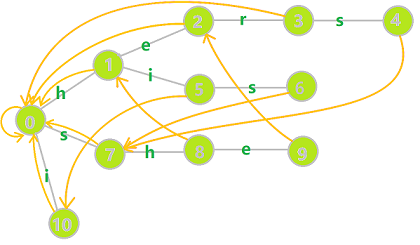
\includegraphics{ac.png}
%\caption{}
%\end{figure}
\begin{figure}[htb] 
\center{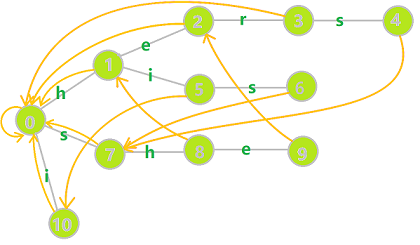
\includegraphics{ac.png}} 
\caption{\label{1} AC自动机示意图} 
\end{figure}

初始将要查询的所有串insert(),之后查询用query()返回匹配到的串的总数。\textbf{千万不要漏了AC.build()}。
\inputminted[linenos]{c++}{string/ac.cpp}

注意以下几点:
\begin{itemize}
  \item AC 自动机求的是允许部分重合的子串出现次数,如果要求求相离的子串出现次数,可以通过记录上一个出现位置来判断。
  \item 该版本代码无法处理查询相同的子串(后面会覆盖前面),可以通过判断来支持。
\end{itemize}

\inputminted[linenos]{c++}{string/acplus.cpp}


% SA
\subsection{后缀数组SA}
\subsubsection{SA求解}
\paragraph{倍增}
\inputminted[linenos]{c++}{string/sabeizeng.cpp}
\paragraph{SA-IS}
摘自\href{https://riteme.site/blog/2016-6-19/sais.html}{诱导排序与 SA-IS 算法}
\inputminted[linenos,breaklines]{c++}{string/sais.cpp}

\subsubsection{height数组}
\paragraph{基本定义}

\(lcp(u,v)\) 代表 \(u,v\) 两个字符串的最长公共前缀长度。

\(LCP(i,j)\) 第 \(i\) 个后缀与第 \(j\) 个后缀的最长公共前缀长度。

\(height[i]=lcp(sa[i],sa[i-1])\) 排名 \(i\)
与其前一名后缀的最长公共前缀长度。

\(h[i]=height[rank[i]]\) 后缀 \(i\)
和排序后在他前一名的后缀的最长公共前缀长度。

重要性质:\(h[i]\ge h[i-1]-1\)

\paragraph{height数组求解 \(O(n)\)}
\inputminted[linenos,breaklines]{c++}{string/height.cpp}

\paragraph{性质与应用}

\begin{itemize}
\item
  \(lcp(sa[i],sa[j])=\min\lbrace{height[i+1\dots j]}\rbrace\)

\item
  比较字符串关系:

  \(A=S[a\dots b],B=[c\dots d]\)

  \(if\ lcp(a,c)>\min\lbrace{|A|,|B|}\rbrace,then\ A<B\iff |A|<|B|\)

  \(else\ A<B\iff rk[a]<rk[b]\)

\item
  不同子串数目:后缀的前缀,考虑枚举后缀,统计前缀。

  前缀总数=子串总数=\(\frac{n(n+1)}{2}\)

  考虑去掉重复的:以每个后缀开始,重复了lcp个。

  答案:\(\frac{n(n+1)}{2}-\sum\limits_{i=2}^{n}height[i]\)
\end{itemize}

% SAM
\subsection{后缀自动机SAM}
\subsubsection{原理与实现}

一个字符串 \(S\) 的自动机接受且仅接受 \(S\) 的后缀。

对于一个状态 \(st\) ,只保存以下要素:

\begin{longtable}[]{@{}ll@{}}
\toprule
数据 & 含义\tabularnewline
\midrule
\endhead
\(maxlen(st)\) & \(st\) 包含的最长子串长度\tabularnewline
\(trans[st][\sum c]\) & \(st\) 的转移函数,其中 \(\sum c\)
为字符集\tabularnewline
\(link[st]\) & \(st\) 的后缀链接\tabularnewline
\bottomrule
\end{longtable}

可能用到的性质:

0.在 \(|S|\ge 3\) 时, 总状态数不超过 \(2\times |S|-1\),转移数不超过
\(3\times|S|-4\) 

1.对于两个不同状态u和v,包含的子串substrings(u),substrings(v)的交为空集; 

2.每个子串都恰好被一个状态包含。

3.minlen(st)=maxlen(link(st))+1

注:代码中的拓扑排序用来计算每个状态 st 的 endpos 大小 cnt[st],也即该类子串出现了几次。别忘了初始化 SAM::init()。

\inputminted[linenos]{c++}{string/sam.cpp}

\subsubsection{应用}
\begin{itemize}
\item
  求 S 的不同字串:对所有 st 求 \(\sum_{st}maxlen(st)-minlen(st)+1\)
\item
  求子串的出现次数:每个子串存在且仅存在于一个状态 st 中,统计其 st 的 endpos 大小即是出现次数。而 endpos 大小为所有以他为 link 的 st 的和(如果包含原字符串前缀,即初始加入不用复制的状态,+1)。所以可以通过加入时标记(vis),拓扑排序计算。

衍生:求长度为 K 子串中出现次数最多的子串的出现次数。设长度为 x 的答案为 ans[x],考虑到随 x 增大 ans[x] 单调递减,只需要通过更新每个 st 的最大值,然后对每个 ans 更新 ans[x]=max(ans[x],ans[x+1]) 即可。

\begin{minted}{cpp}
void getans(){
    for (int i=1;i<=sz;++i){
        ans[st[i].mxlen]=max(ans[st[i].mxlen],cnt[i]);
    }
    for (int i=len-1;i>=1;--i){
        ans[i]=max(ans[i+1],ans[i]);
    }
}
\end{minted}

\end{itemize}

% Manacher
\subsection{Manacher}
最长回文串,复杂度\(O(N)\)。

一般将初始字符串左右端加上特殊字符,同时每个字符之间插上\textbf{同一特殊字符}'\#'
\inputminted[linenos]{c++}{string/manacher.cpp}
% 字符串end


\newpage
% 动态规划start
\section{动态规划}
% 线性dp
\subsection{线性DP}
\subsubsection{LIS 问题}
用d数组存储目前的最长上升or下降子序列。
\inputminted[linenos]{c++}{dp/lis.cpp}
% 背包dp
\subsection{背包DP}
去看\textbf{《背包九讲》}即可。
% 区间dp
\subsection{区间DP}
\textbf{合并} :即将两个或多个部分进行整合,当然也可以反过来。

\textbf{特征} :能将问题分解为能\textbf{两两合并}的形式。如果是 \(k\)
个合并在一块,且\textbf{能转化为 1 个和 k-1
个合并的形式},也是可以利用的。

\textbf{求解}
:对整个问题设最优值,枚举合并点,将问题分解为左右两个部分,最后合并两个部分的最优值得到原问题的最优值。

\textbf{例题:}\(n\) 堆石子,一次只能合并\textbf{连续}的 \([l,r]\)
堆。合并价值为数量,求最小耗费。如果无法实现输出 0。

设 \(f[i][j][k]\) 代表从 \(i\) 到 \(j\) 合并了 \(k\)
堆的最小花费,则得到下列表达式:

(1)\(f[i][j][1]=min\lbrace f[i][j][d]+sum[j]-sum[i-1] \rbrace,d\in[l,r]\)
。能直接合并成一堆的肯定比两次合并更优。

(2)\(f[i][j][k]=min\lbrace f[i][x][1]+f[x+1][j][k-1] \rbrace\) 。每一个
\(k\) 堆可以拆成 \(1\) 堆与 \(k-1\) 堆的合并,相当于两两合并。

至于为什么不考虑由 \(d\) 堆和 \(k-d\) 堆合并:枚举 \(d\)
堆明显增加一维复杂度。如果枚举 \(f[i][x][d]\) ,其实相当于内部空间再由
\(f[i][x'][1]+f[x'][x][d-1]\) 组合而成的。也就是说,分成 \(1\) 和
\(k-1\) 实则已经考虑了所有情况,再重复枚举多余。
\inputminted[linenos]{c++}{dp/rangedp.cpp}

% 数位dp
\subsection{数位dp}
关于数字相关的问题考虑数位dp。利用前缀和的思想处理l到r区间个数问题。

例题:从1-n每个数出现了几次。
\inputminted[linenos]{cpp}{dp/shuwei.cpp}

% dp优化
\subsection{动态规划的优化}
% 单调队列
\subsubsection{单调队列,单调栈优化}
\paragraph{多重背包的优化}
单调队列可以优化多重背包:有n个物品,每个物品重 \(w_i\) ,价值 \(v_i\) ,数量 \(k_i\) ,背包重量上限m,求最大价值。

初始方程:\(f_{i,j}=\max\limits_{k=0}^{k_i}\lbrace{f_{i-1,j-k\times w_i}+v_i\times k}\rbrace\) 。复杂度 \(O(nW\sum k_i)\) 。

优化:设 \(g_{x,y}=f_{i,x\times w_i+y},g^{'}_{x,y}=f_{i-1,x\times w_i+y}\) ,得到转移方程: 
\(g_{x,y}=\max\limits_{k=0}^{k_i}\lbrace{g^{'}_{x-k,y}+v_i\times k}\rbrace\)
。不妨设 
\(G_{x,y}=g^{'}_{x,y}-v_i\times x\)
,则方程可以表示为:

\(g_{x,y}=\max\limits_{k=0}^{k_i}\lbrace{G_{x-k,y}}\rbrace+v_i\times x\)

其中 \(G_{x,y}\) 计算为常数,对于固定的y我们可以在 \(O(\frac{W}{w_i})\) 时间内计算出 \(g_{x,y}\) ,求出所有g总时间复杂度为 \(O(\frac{W}{w_i})\times O(w_i)=O(w)\) 。转移总复杂度 \(O(nW)\) 。
% 斜率优化
\subsubsection{斜率优化}

\paragraph{适用类型}

对于转移方程 dp[i]=min/max\{dp[j]+f(j)+g(i)\} ,我们可以通过移项(把关于i的放外面,关于j的在内部)和维护最小值(单点or单调队列)实现 \(O(1)\) 转移。

对于转移方程 dp[i]=min/max\{dp[j]+f(i,j)\} ,由于涉及了i和j,所以不能拆开。考虑使用斜率优化。

\paragraph{两种思路}

解决斜率优化问题考虑两种思路。

\subparagraph{代数}
考虑i确定时,两个决策点 \(0\le j_1< j_2\) ,且后者 \(j_2\) 优于 \(j_1\)。我们假设取小为优,那么可以得到以下方程:
\(dp[j_1]+f(i,j_1)\ge dp[j_2]+f(i,j_2)\)
通过移项等操作,最终能化为
\(h(i)\ge\frac{F(j_1)-F(j_2)}{G(j_1)-G(j_2)}\)
的形式。(h(i)为关于i的常数项,F(j)包含有dp[j]项,G(j)为关于j的常数项,大于小于号不确定)。

确定好优劣之后,我们不妨找到三个决策点A<B<C, AB斜率K1,BC斜率K2,K0=h(i)。若K2<K1,分情况讨论最优(>代表优于):

\begin{itemize}
  \item (1)K0<K2<K1:A>B>C
  \item (2)K2<=K0<K1:A>B,C>B
  \item (3)K2<K1<K0:C>B>A
\end{itemize}

结果无论如何 B 都不是最优决策点,于是便可以删除该点。

最终可以看出,最优决策点组成了上or下凸包,其斜率递增or减。关键在于维护凸包。

\subparagraph{线性规划}

将原方程 dp[i]=min/max\{dp[j]+f(i,j)\} 转化为 y=kx+b 的模式,其中 f(i,j)看做斜率k乘x(k为i相关,x为j相关),dp[i]作为目标在b中(出去第一步与i相关的所有值也在内),y代表所有与j相关的值(包括dp[j])。若x的表达式单调递减,推荐两端同乘-1使其单增。

最小化dp[i]可以转化为最小化b,斜率一定时,使得b最小化的点也在凸包中。

\subparagraph{两种结合}
两种方法结合来看。

线性规划表示十分直观,且在某变量不满足单调性时能快速判断。通过线性规划也可以看出,\textbf{最优决策点的左右两边斜率符号相反,自身为极大or小值,}可以通过二分得到。

代数法可以转换思维方向,通过斜率比较方便去点。

\paragraph{决策单调性的结合}
一般而言,通过单调队列维护凸包点集。复杂度 \(O(n\log n)\) 。
\begin{itemize}
  \item (1) 在凸包上找到最优决策点j。
  \item (2) 通过j更新dp[i]。
  \item (3) 将i作为决策点加入。
  \item 注:若i为dp[i]的决策点,则(3)放在第一步。
\end{itemize}

如果具有决策单调性,即最优决策点递增。我们在更新dp[i]的时候,可以以i为媒介从尾部挨个枚举两个元素j和j-1,确定是否删除j-1。找到的第一个满足j-1优于j的点j-1便是最优决策点。在加入一个新点的时候,为了满足凸包,在头部删除。每个元素入队出队一次,复杂度 \(O(n)\) 。

代码:玩具装箱
\begin{minted}[breaklines]{cpp}
double k(int i,int j){
    return ((double)(f[i]-f[j]+(i+s[i])*(i+s[i])-(j+s[j])*(j+s[j]))
             /(double)(2.0*(i+s[i]-j-s[j])));
}
//main
head=tail=1; q[1]=0;
    for (int i=1;i<=n;++i){
        while (head<tail&&
                 k(q[head],q[head+1])<=(double)(i-1-l+s[i])) 
                 head++;
        f[i]=f[q[head]]
            +(i-q[head]-1-l+s[i]-s[q[head]])
            *(i-q[head]-1-l+s[i]-s[q[head]]);
        while (head<tail&&
                 k(q[tail-1],q[tail])>=k(q[tail],i)) tail--;
        q[++tail]=i;
}
\end{minted}
注意事项:
\begin{itemize}
\item 先判断能不能用斜率优化,即写成 \(\frac{Y(j_2)-Y(j_1)}{X(j_2)-X(j_1)}\) 的形式。
\item 注意判断上凸还是下凸。
\item 若存在X(j)相等的情况,注意设INF且注意符号问题。如果用叉积解决的话可以解除干扰。比较斜率是推荐不等式中包含等号,解决重复问题。
\item 注意初始点的问题,可能不为0。
\item 斜率最好使用精度高的long double,或者使用向量叉积解决。
\end{itemize}
\paragraph{单调性相关讨论}
\subparagraph{决策点横坐标X(j)单调}
最方便处理的类型,直接单调队列 \(O(n)\) 解决。
\subparagraph{决策点横坐标X(j)不单调}
不能使用单调队列,通过平衡树或者CDQ分治维护凸包单调性。
\subparagraph{待决策点h(i)函数(或理解为斜率)不单调}
不保证具有决策单调性,不能弹走队首,同时答案也不能直接是队首,需要二分。

代码:任务安排。
\inputminted[linenos]{c++}{dp/xielv.cpp}
\subparagraph{X(j),h(i)都不单调}
利用平衡树维护凸包,通过平衡树也能方便查到h(i)的前驱后继。如果用CDQ需加一维偏序。
% 四边形不等式优化
\subsubsection{四边形不等式优化}
% 2D1D
\paragraph{2D1D(区间类)动态规划应用}

如以下形式的转移方程:
\(f_{l,r}=\min\limits_{k=l}^{r-1}\lbrace{f_{l,k}+f_{k+1,r}}\rbrace+w(l,r)\) 

朴素转移 \(O(n^3)\) ,但若 \(w(l,r)\) 满足以下性质时,我们可以通过\textbf{决策单调性}进行优化。(\textbf{决策单调性}:随状态增大,最优决策点非严格递增。)
\begin{itemize}
\item 1.\textbf{区间包含单调性}:对于任意 \(l\le l^{'}\le r^{'}\le r\) ,都有 \(w(l^{'},r^{'})\le w(l,r)\)。
\item 2.\textbf{四边形不等式}:对于任意 \(l_1\le l_2\le r_1\le r_2\) ,都有 \(w(l_1,r_1)+w(l_2,r_2)\le w(l_1,r_2)+w(l_2,r_1)\) 成立。
\end{itemize}

相关定理:
\begin{itemize}
  \item \(w(l,r)\) 满足区间包含单调性的同时满足四边形不等式,则 \(f_{l,r}\) 也满足四边形不等式。
  \item 若f满足四边形不等式,记 \(m_{l,r}=\min\lbrace{k:f_{l,r}=f_{l,k}+f_{k+1,r}+w(l,r)}\rbrace\) 表示最优决策点,则
\(m_{l,r-1}\le m_{l,r}\le m_{l+1,r}\) 。
\end{itemize}

因此在计算 \(f_{l,r}\) 的时候可以记录最优决策点 \(m_{l,r}\) ,那么对决策点k的枚举总量就将为 \(n^2\) 。
\begin{minted}{cpp}
for (int len=2;len<=n;++len){
    for (int l=1,r=len;r<=len;++l,--r){
        f[l][r]=INF;
        for (int k=m[l][r-1];k<=m[l+1][r];++k){
            if (f[l][r]>f[l][r]+f[k+1][r]+w(l,r)){
                f[l][r]=f[l][k]+f[k+1][r]+w(l,r);
                m[l][r]=k;
            }
        }
    }
}
\end{minted}
% 1D1D
\paragraph{1D1D动态规划应用}

如以下形式的转移方程:
\(f_r=\min\limits_{l=1}^{r-1}\lbrace{f_l+w(l,r)}\rbrace\)

若函数 \(w(l,r)\) 满足四边形不等式,记 \(m_r=\min\lbrace{l|f_r=f_l+w(l,r)}\rbrace\) ,则 
\(\forall r_1<r_2:k_{r_1}\le k_{r_2}\)。

我们只能得知枚举l的下界但无法确定上界。但可以解决一种特殊情况:
\(f_r=\min\limits_{l=1}^{r-1}\lbrace{w(l,r)}\rbrace\) 。我们定义 \(dp(l,r,k_l,k_r)\) 表示求 \(f_l\to f_r\) 的状态值,并且知道其最优决策点必然在 \([k_l,k_r]\) 中,可以使用分治算法解决。复杂度 \(O(n\log n)\) 。

\begin{minted}{cpp}
void dp(int l,int r,int kl,int kr){
    int mid=(l+r)>>1,k=kl;
    for (int i=kl;i<=min(kr,mid-1);++i){
        if (w(i,mid)<w(k,mid)) i=k;
    }
    f[mid]=w(k,mid);
    if (l<mid) dp(l,mid-1,kl,k);
    if (r>mid) dp(mid+1,r,k,k_r);
}
\end{minted}

% 四边形不等式函数类
\paragraph{满足四边形不等式的常见性质}
\begin{itemize}
\item
  若 \(w_1(l,r)\) 和 \(w_2(l,r)\) 同时满足四边形不等式(或区间包含单调性),则 \(c_1w_1+c_2w_2\) 同样满足四边形不等式(或区间包含单调性)(\(c_1\ge 0,c_2\ge 0\))
\item
  若存在函数 \(f(x),g(x)\) 满足 \(w(l,r)=f(r)-g(l)\) ,则 \(w(l,r)\) 满足四边形恒等式(四边形不等式不等号变等号)。当函数 \(f(x),g(x)\) 单调增加时,函数 \(w(l,r)\) 还满足区间包含单调性。
\item
  设 \(h(x)\) 是一个单增的凸函数(下凸函数,导数单调增加),若函数 \(w(l,r)\) 满足四边形不等式且区间包含单调性,则函数 \(h(w(l,r))\) 满足四边形不等式且区间包含单调性。
\item
  设 \(h(x)\) 是一个凸函数,若函数 \(w(l,r)\) 满足四边形不等式且区间包含单调性,则函数 \(h(w(l,r))\) 满足四边形不等式。
\end{itemize}
% 动态规划end


%\newpage
%\section{Others}

\end{document}
